\documentclass{standalone}
\usepackage{tikz}
\usetikzlibrary{patterns, positioning}
\usepackage[sfdefault]{ClearSans} %% option 'sfdefault' activates Clear Sans as the default text font
\usepackage[T1]{fontenc}

\begin{document}
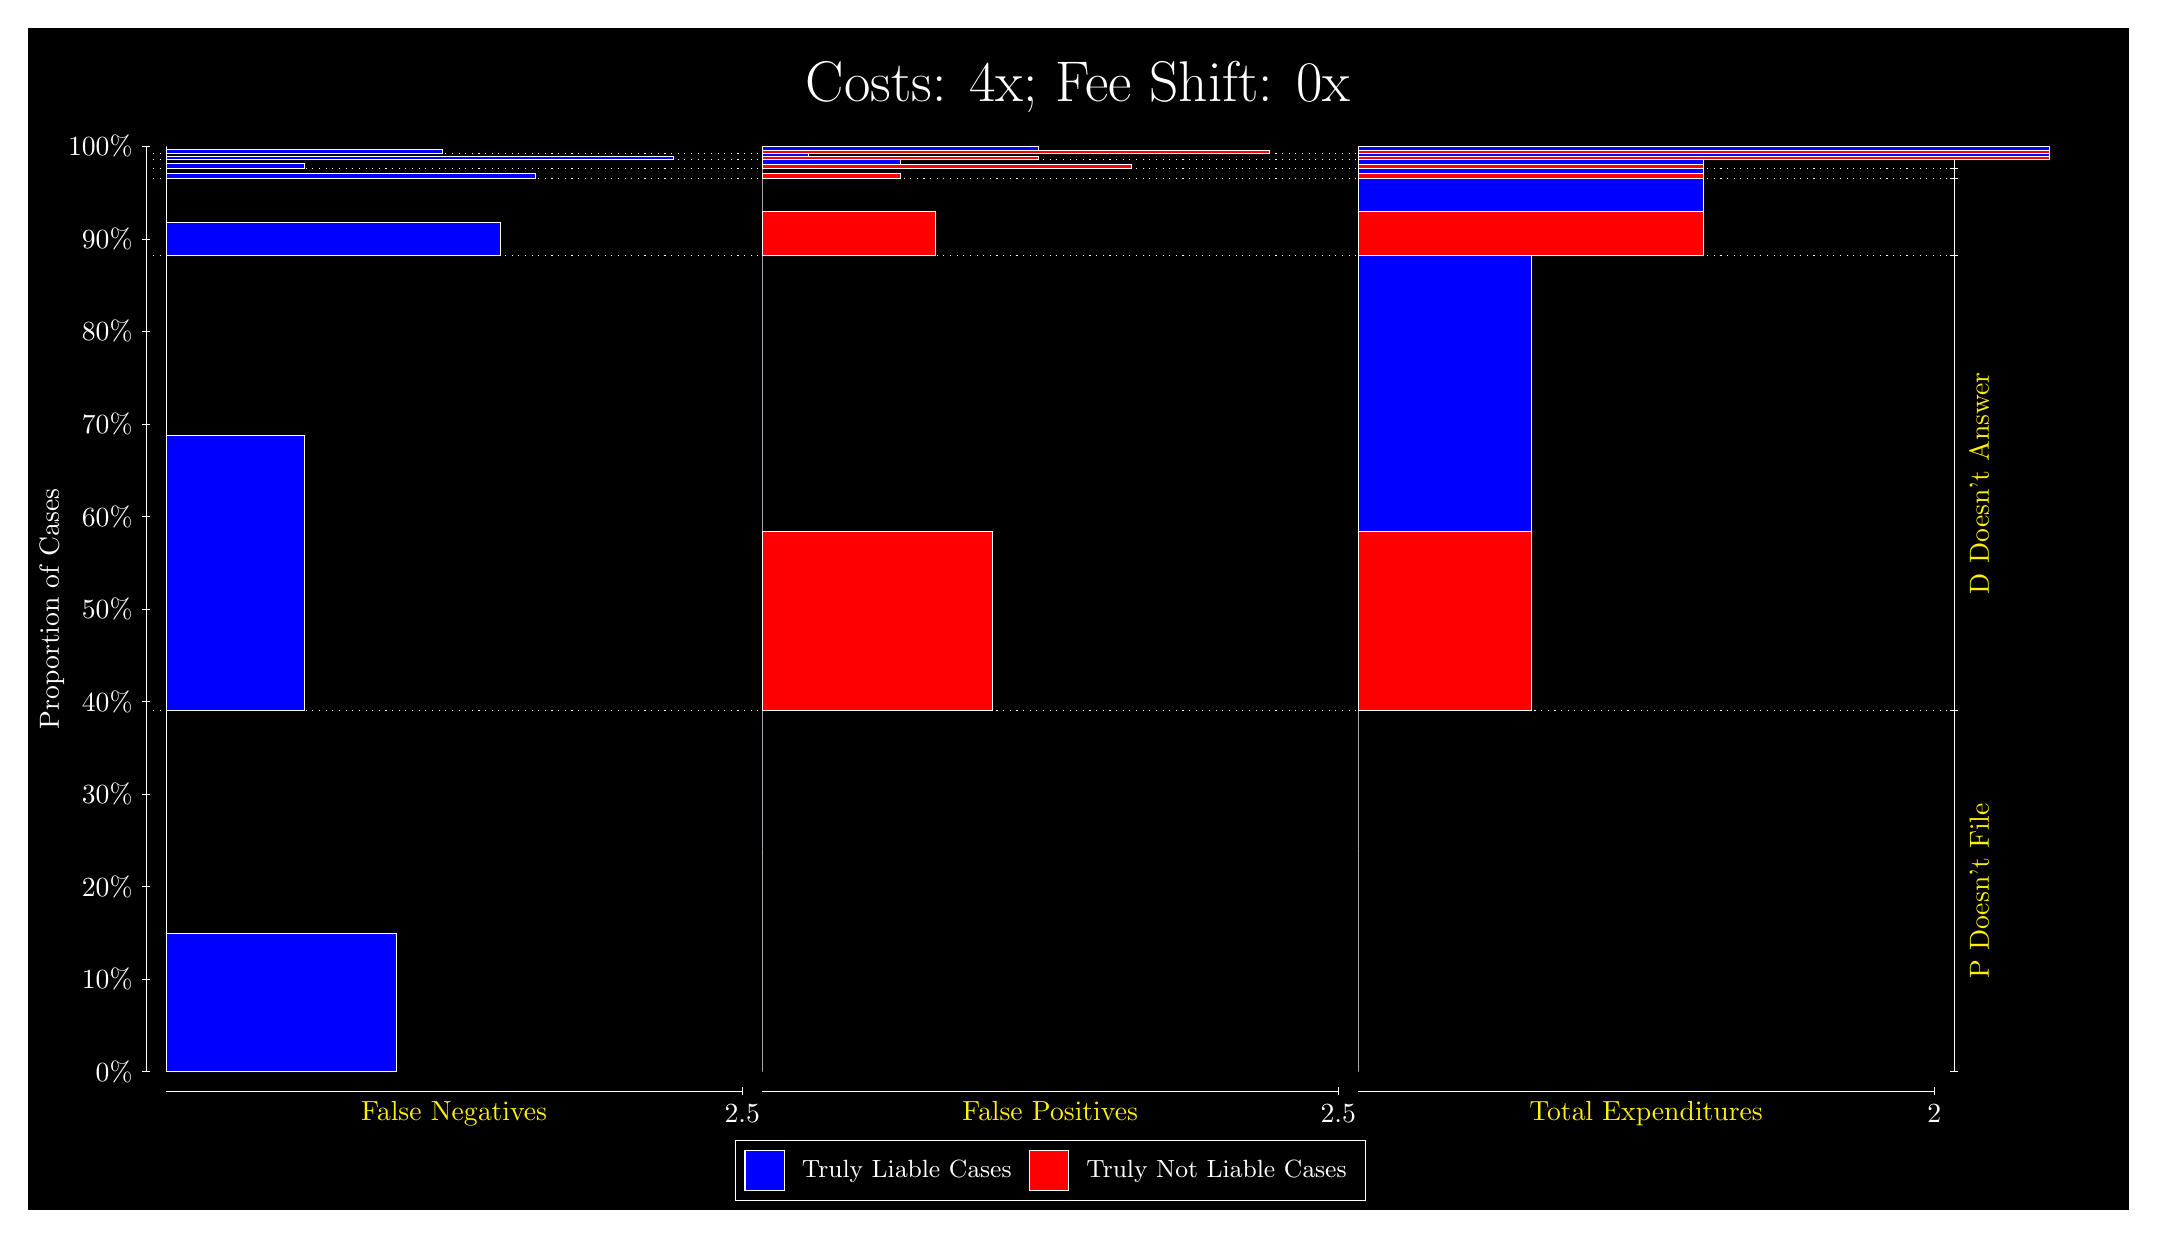
\begin{tikzpicture}
\draw[fill=black] (0,0) rectangle (26.667,15);
\draw[text=white] (0,13.5) rectangle (26.667,15) node[midway] {\huge Costs: 4x; Fee Shift: 0x};
\draw[white, very thin] (1.5,1.75) -- (1.5,13.5);
\node[rotate=90, text=white, anchor=center] at (0.3, 7.625) {Proportion of Cases};
\draw[white, very thin] (1.45,1.75) -- (1.55,1.75);
\node[text=white, anchor=east] at (1.45, 1.75) {0\%};
\draw[white, very thin] (1.45,2.925) -- (1.55,2.925);
\node[text=white, anchor=east] at (1.45, 2.925) {10\%};
\draw[white, very thin] (1.45,4.1) -- (1.55,4.1);
\node[text=white, anchor=east] at (1.45, 4.1) {20\%};
\draw[white, very thin] (1.45,5.275) -- (1.55,5.275);
\node[text=white, anchor=east] at (1.45, 5.275) {30\%};
\draw[white, very thin] (1.45,6.45) -- (1.55,6.45);
\node[text=white, anchor=east] at (1.45, 6.45) {40\%};
\draw[white, very thin] (1.45,7.625) -- (1.55,7.625);
\node[text=white, anchor=east] at (1.45, 7.625) {50\%};
\draw[white, very thin] (1.45,8.8) -- (1.55,8.8);
\node[text=white, anchor=east] at (1.45, 8.8) {60\%};
\draw[white, very thin] (1.45,9.975) -- (1.55,9.975);
\node[text=white, anchor=east] at (1.45, 9.975) {70\%};
\draw[white, very thin] (1.45,11.15) -- (1.55,11.15);
\node[text=white, anchor=east] at (1.45, 11.15) {80\%};
\draw[white, very thin] (1.45,12.325) -- (1.55,12.325);
\node[text=white, anchor=east] at (1.45, 12.325) {90\%};
\draw[white, very thin] (1.45,13.5) -- (1.55,13.5);
\node[text=white, anchor=east] at (1.45, 13.5) {100\%};

\draw[white, very thin] (24.457,1.75) -- (24.457,13.5);
\draw[white, very thin] (24.407,1.75) -- (24.507,1.75);
\node[anchor=west] at (24.407, 1.75) {};
\draw[white, very thin] (24.407,6.3347) -- (24.507,6.3347);
\node[anchor=west] at (24.407, 6.3347) {};
\draw[white, very thin] (24.407,12.111) -- (24.507,12.111);
\node[anchor=west] at (24.407, 12.111) {};
\draw[white, very thin] (24.407,13.097) -- (24.507,13.097);
\node[anchor=west] at (24.407, 13.097) {};
\draw[white, very thin] (24.407,13.22) -- (24.507,13.22);
\node[anchor=west] at (24.407, 13.22) {};
\draw[white, very thin] (24.407,13.334) -- (24.507,13.334);
\node[anchor=west] at (24.407, 13.334) {};
\draw[white, very thin] (24.407,13.413) -- (24.507,13.413);
\node[anchor=west] at (24.407, 13.413) {};
\draw[white, very thin] (24.407,13.5) -- (24.507,13.5);
\node[anchor=west] at (24.407, 13.5) {};

\draw[white, very thin, fill=blue] (1.75,1.75) rectangle (4.6775,3.5035);
\draw[white, very thin, fill=red] (1.75,3.5035) rectangle (1.75,6.3347);
\draw[white, very thin, fill=blue] (1.75,6.3347) rectangle (3.5065,9.832);
\draw[white, very thin, fill=red] (1.75,9.832) rectangle (1.75,12.111);
\draw[white, very thin, fill=blue] (1.75,12.111) rectangle (5.9949,12.532);
\draw[white, very thin, fill=red] (1.75,12.532) rectangle (1.75,13.097);
\draw[white, very thin, fill=blue] (1.75,13.097) rectangle (6.4341,13.154);
\draw[white, very thin, fill=red] (1.75,13.154) rectangle (1.75,13.22);
\draw[white, very thin, fill=blue] (1.75,13.22) rectangle (3.5065,13.281);
\draw[white, very thin, fill=red] (1.75,13.281) rectangle (1.75,13.334);
\draw[white, very thin, fill=blue] (1.75,13.334) rectangle (8.1906,13.371);
\draw[white, very thin, fill=red] (1.75,13.371) rectangle (1.75,13.413);
\draw[white, very thin, fill=blue] (1.75,13.413) rectangle (5.2631,13.461);
\draw[white, very thin, fill=red] (1.75,13.461) rectangle (1.75,13.5);
\draw[white, very thin, fill=red] (9.3189,1.75) rectangle (9.3189,4.5812);
\draw[white, very thin, fill=blue] (9.3189,4.5812) rectangle (9.3189,6.3347);
\draw[white, very thin, fill=red] (9.3189,6.3347) rectangle (12.246,8.6138);
\draw[white, very thin, fill=blue] (9.3189,8.6138) rectangle (9.3189,12.111);
\draw[white, very thin, fill=red] (9.3189,12.111) rectangle (11.515,12.676);
\draw[white, very thin, fill=blue] (9.3189,12.676) rectangle (9.3189,13.097);
\draw[white, very thin, fill=red] (9.3189,13.097) rectangle (11.075,13.162);
\draw[white, very thin, fill=blue] (9.3189,13.162) rectangle (9.3189,13.22);
\draw[white, very thin, fill=red] (9.3189,13.22) rectangle (14.003,13.273);
\draw[white, very thin, fill=blue] (9.3189,13.273) rectangle (11.075,13.334);
\draw[white, very thin, fill=red] (9.3189,13.334) rectangle (12.832,13.376);
\draw[white, very thin, fill=blue] (9.3189,13.376) rectangle (9.9044,13.413);
\draw[white, very thin, fill=red] (9.3189,13.413) rectangle (15.759,13.452);
\draw[white, very thin, fill=blue] (9.3189,13.452) rectangle (12.832,13.5);
\draw[white, very thin, fill=red] (16.888,1.75) rectangle (16.888,4.5812);
\draw[white, very thin, fill=blue] (16.888,4.5812) rectangle (16.888,6.3347);
\draw[white, very thin, fill=red] (16.888,6.3347) rectangle (19.083,8.6138);
\draw[white, very thin, fill=blue] (16.888,8.6138) rectangle (19.083,12.111);
\draw[white, very thin, fill=red] (16.888,12.111) rectangle (21.279,12.676);
\draw[white, very thin, fill=blue] (16.888,12.676) rectangle (21.279,13.097);
\draw[white, very thin, fill=red] (16.888,13.097) rectangle (21.279,13.162);
\draw[white, very thin, fill=blue] (16.888,13.162) rectangle (21.279,13.22);
\draw[white, very thin, fill=red] (16.888,13.22) rectangle (21.279,13.273);
\draw[white, very thin, fill=blue] (16.888,13.273) rectangle (21.279,13.334);
\draw[white, very thin, fill=red] (16.888,13.334) rectangle (25.67,13.376);
\draw[white, very thin, fill=blue] (16.888,13.376) rectangle (25.67,13.413);
\draw[white, very thin, fill=red] (16.888,13.413) rectangle (25.67,13.452);
\draw[white, very thin, fill=blue] (16.888,13.452) rectangle (25.67,13.5);
\draw[white, dotted] (1.5,6.3347) -- (24.457,6.3347);
\draw[white, dotted] (1.5,12.111) -- (24.457,12.111);
\draw[white, dotted] (1.5,13.097) -- (24.457,13.097);
\draw[white, dotted] (1.5,13.22) -- (24.457,13.22);
\draw[white, dotted] (1.5,13.334) -- (24.457,13.334);
\draw[white, dotted] (1.5,13.413) -- (24.457,13.413);
\draw[white, very thin] (1.75,1.5) -- (9.0689,1.5);
\node[text=yellow, anchor=north] at (5.4094, 1.5) {False Negatives};
\draw[white, very thin] (9.0689,1.45) -- (9.0689,1.55);
\node[text=white, anchor=north] at (9.0689, 1.45) {2.5};

\draw[white, very thin] (9.3189,1.5) -- (16.638,1.5);
\node[text=yellow, anchor=north] at (12.978, 1.5) {False Positives};
\draw[white, very thin] (16.638,1.45) -- (16.638,1.55);
\node[text=white, anchor=north] at (16.638, 1.45) {2.5};

\draw[white, very thin] (16.888,1.5) -- (24.207,1.5);
\node[text=yellow, anchor=north] at (20.547, 1.5) {Total Expenditures};
\draw[white, very thin] (24.207,1.45) -- (24.207,1.55);
\node[text=white, anchor=north] at (24.207, 1.45) {2};

\node[text=yellow, centered, rotate=90] at (24.777, 4.0424) {P Doesn't File};
\node[text=yellow, centered, rotate=90] at (24.777, 9.2229) {D Doesn't Answer};






\draw (12.978300999999998,1.5) node[draw=none] (baseCoordinate) {};
\begin{scope}[align=center]
        \matrix[scale=0.5, draw=white, below=0.5cm of baseCoordinate, nodes={draw}, column sep=0.1cm]{
            \node[rectangle, draw, minimum width=0.5cm, minimum height=0.5cm, fill=blue] {}; &
            \node[draw=none, font=\small, text=white] (B) {Truly Liable Cases}; &
            \node[rectangle, draw, minimum width=0.5cm, minimum height=0.5cm, fill=red] {}; &
            \node[draw=none, font=\small, text=white] (B) {Truly Not Liable Cases}; \\
            };
\end{scope}

\end{tikzpicture}
\end{document}